\subsection{Caso d'uso UC7: Gestione delle domande}
	
\subsubsection{UC7.1 - Creazione nuova domanda}
	\begin{center}
		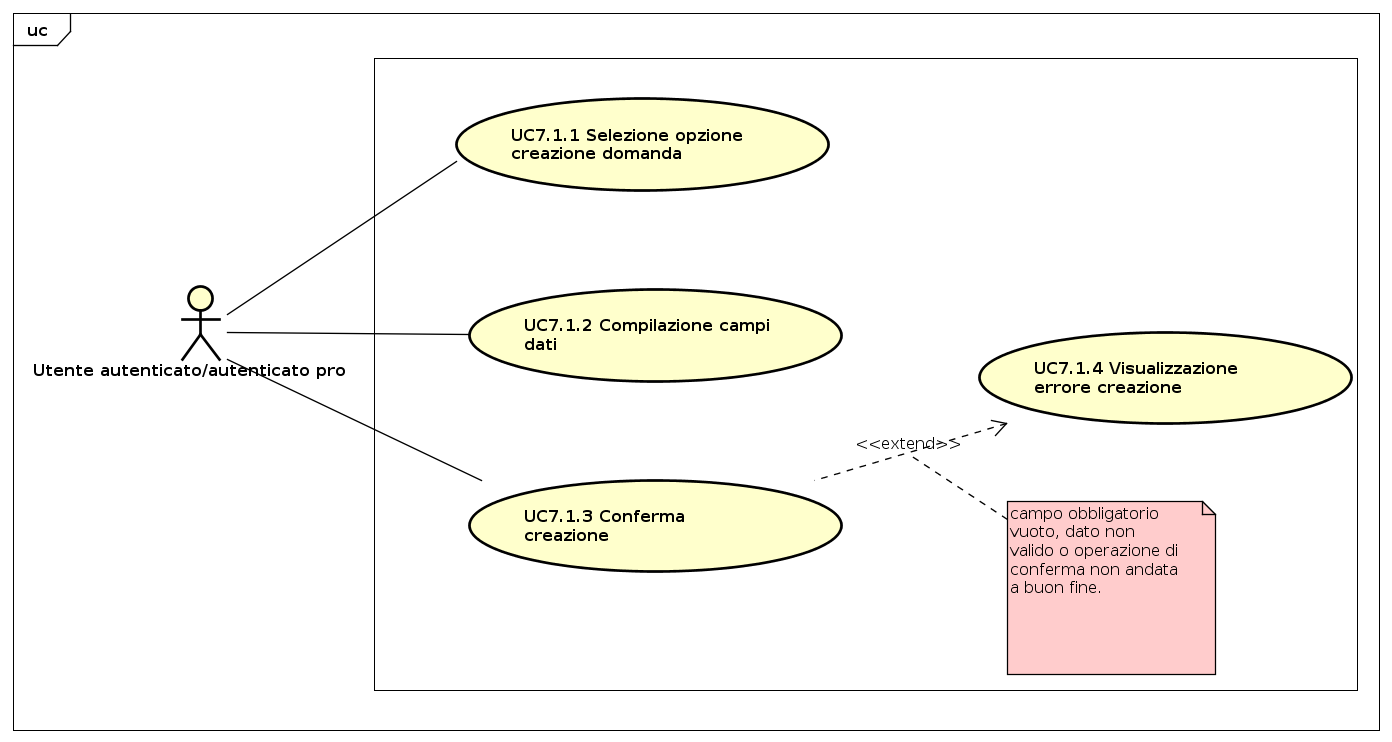
\includegraphics[scale=0.5]{UML/UC7.1.png}
	\end{center}
	\begin{itemize}
		\item
			\textbf{Attori}: utente autenticato, utente autenticato pro;
		\item		
			\textbf{Scopo e descrizione}: L'utente autenticato crea una nuova domanda nel db, utile all'apprendimento di un certo argomento;
		\item
			\textbf{Pre-condizione}: L'utente è autenticato presso il sistema. 
		\item
			\textbf{Flusso principale degli eventi}:
	       		\begin{enumerate}
					\item 	
					L'utente seleziona l'opzione per la creazione della domanda [UC7.1.1];
					\item
					L'utente compila i campi dati del modulo previsto per compiere questa operazione [UC7.1.2];
					\item
					L'utente conferma la creazione della domanda [UC7.1.3];
	 			\end{enumerate}
	 	\item
	 		\textbf{Scenario alternativo}: possono verificarsi uno o più di questi scenari:
				\begin{itemize}
					\item[-] 	
						E' presente un campo obbligatorio vuoto;
					\item[-] 
    						E' presente  un dato non valido;
					\item[-] 
						L'operazione di conferma non è andata a buon fine.
				\end{itemize}
			In tal caso il sistema ripresenta il modulo di creazione della domanda, presentando un messaggio d'errore.
		\item
			\textbf{Estensione}: L'utente visualizza un messaggio d'errore di conferma [UC7.1.4].
		\item
			\textbf{	Post-condizione}: L'utente riceve conferma dell'avvenuta creazione.
	\end{itemize}
	\subsubsection{UC7.1.1 - Selezione opzione creazione domanda}
	\begin{itemize}
		\item
			\textbf{Attori}: utente autenticato, utente autenticato pro;
		\item
			\textbf{Scopo e descrizione}: l'utente autenticato seleziona l'opzione per la creazione di una domanda;
		\item		
			\texbf{Pre-condizione}: il sistema presenta all'utente autenticato l'opzione per compiere questa operazione;
		\item
			\texbf{Post-condizione}: il sistema presenta all'utente autenticato il modulo per creare la domanda.
	\end{itemize}	
	\subsubsection{UC7.1.2 - Compilazione campi dati}
	\begin{itemize}
		\item
			\textbf{Attori}: utente autenticato, utente autenticato pro;
		\item
			\textbf{Scopo e descrizione}: l'utente autenticato compila i campi dati del modulo per la creazione della domanda;
		\item		
			\texbf{Pre-condizione}: il sistema presenta all'utente autenticato ha selezionato l'opzione per creare la domanda;
		\item
			\texbf{Post-condizione}: i campi dati del modulo di creazione sono riempiti.
	\end{itemize}	
	\subsubsection{UC7.1.3 - Conferma creazione}
	\begin{itemize}
		\item
			\textbf{Attori}: utente autenticato, utente autenticato pro;
		\item
			\textbf{Scopo e descrizione}: l'utente autenticato conferma la creazione della domanda per essere inserita nel DB;
		\item		
			\texbf{Pre-condizione}: il sistema presenta all'utente autenticato l'opzione per compiere questa operazione;
		\item
			\texbf{Post-condizione}: il sistema ha ricevuto i dati per la registrazione.
	\end{itemize}	
	\subsubsection{UC7.1.4 - Visualizzazione errore creazione}
	\begin{itemize}
		\item
			\textbf{Attori}: utente autenticato, utente autenticato pro;
		\item
			\textbf{Scopo e descrizione}: l'utente visualizza un messaggio d'errore nel caso si fossero verificati uno o più scenari alternativi;
		\item		
			\texbf{Pre-condizione}: il sistema ha ricevuto dei dati errati per creazione;
		\item
			\texbf{Post-condizione}: il sistema mostra un messaggio d'errore.
	\end{itemize}	
	\subsubsection{UC7.2 - Modifica domanda esistente}
	\begin{center}
		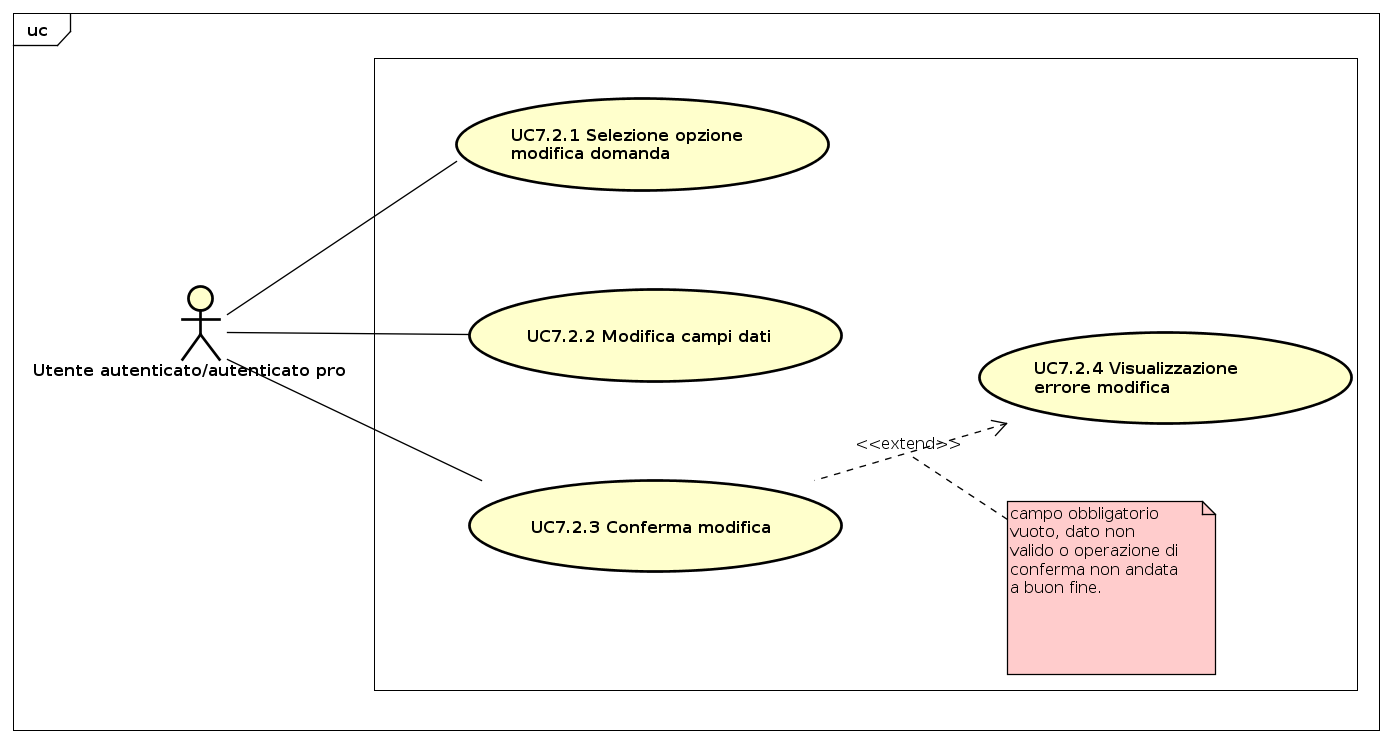
\includegraphics[scale=0.5]{UML/UC7.2.png}
	\end{center}
	\begin{itemize}
		\item
			\textbf{Attori}: utente autenticato, utente autenticato pro;
		\item		
			\textbf{Scopo e descrizione}: L'utente autenticato modifica una domanda da lui in precedenza creata per correggere errori ortografici o sintattici;
		\item
			\textbf{Pre-condizione}: L'utente è autenticato presso il sistema. 
		\item
			\textbf{Flusso principale degli eventi}:
	       		\begin{enumerate}
					\item 	
					L'utente seleziona l'opzione per la modifica della domanda [UC7.2.1];
					\item
					L'utente modifica i campi dati, già precompilati dai dati della domanda selezionata, del modulo previsto per compiere questa operazione [UC7.2.2];
					\item
					L'utente conferma la modifica della domanda [UC7.2.3];
	 			\end{enumerate}
	 	\item
	 		\textbf{Scenario alternativo}: possono verificarsi uno o più di questi scenari:
				\begin{itemize}
					\item[-] 	
						E' presente un campo obbligatorio vuoto;
					\item[-] 
    						E' presente  un dato non valido;
					\item[-] 
						L'operazione di conferma non è andata a buon fine.
				\end{itemize}
			In tal caso il sistema ripresenta il modulo di modifica della domanda, presentando un messaggio d'errore.
		\item
			\textbf{Estensione}: L'utente visualizza un messaggio d'errore di conferma [UC7.2.4].
		\item
			\textbf{	Post-condizione}: L'utente riceve conferma dell'avvenuta modifica.
	\end{itemize}
	\subsubsection{UC7.2.1 - Selezione opzione modifica domanda}
	\begin{itemize}
		\item
			\textbf{Attori}: utente autenticato, utente autenticato pro;
		\item
			\textbf{Scopo e descrizione}: l'utente autenticato seleziona l'opzione per compiere la modifica della domanda;
		\item		
			\texbf{Pre-condizione}: il sistema presenta all'utente autenticato l'opzione per compiere questa operazione;
		\item
			\texbf{Post-condizione}: il sistema presenta all'utente autenticato il modulo per modificare la domanda.
	\end{itemize}
	\subsubsection{UC7.2.2 - Modifica campi dati}
	\begin{itemize}
		\item
			\textbf{Attori}: utente autenticato, utente autenticato pro;
		\item
			\textbf{Scopo e descrizione}: l'utente autenticato modifica i dati della domanda selezionata;
		\item		
			\texbf{Pre-condizione}: il sistema presenta all'utente autenticato il modulo per modificare la domanda selezionata;
		\item
			\texbf{Post-condizione}: i campi dati del modulo di modifica, già precompilati con i dati della domanda selezionata, sono modificati.
	\end{itemize}		
	\subsubsection{UC7.2.3 - Conferma modifica}
	\begin{itemize}
		\item
			\textbf{Attori}: utente autenticato, utente autenticato pro;
		\item
			\textbf{Scopo e descrizione}: l'utente autenticato conferma la modifica dei dati della domanda selezionata;
		\item		
			\texbf{Pre-condizione}: il sistema presenta all'utente autenticato l'opzione per compiere questa operazione;
		\item
			\texbf{Post-condizione}: il sistema ha ricevuto i dati per la registrazione.
	\end{itemize}		
	\subsubsection{UC7.2.4 - Visualizzazione errore modifica}
	\begin{itemize}
		\item
			\textbf{Attori}: utente autenticato, utente autenticato pro;
		\item
			\textbf{Scopo e descrizione}: l'utente visualizza un messaggio d'errore nel caso si fossero verificati uno o più scenari alternativi;
		\item		
			\texbf{Pre-condizione}: il sistema ha ricevuto dei dati errati per la modifica;
		\item
			\texbf{Post-condizione}: il sistema mostra un messaggio d'errore.
	\end{itemize}	
	
	\subsubsection{UC7.3 - Eliminazione domanda}	
	\begin{center}
		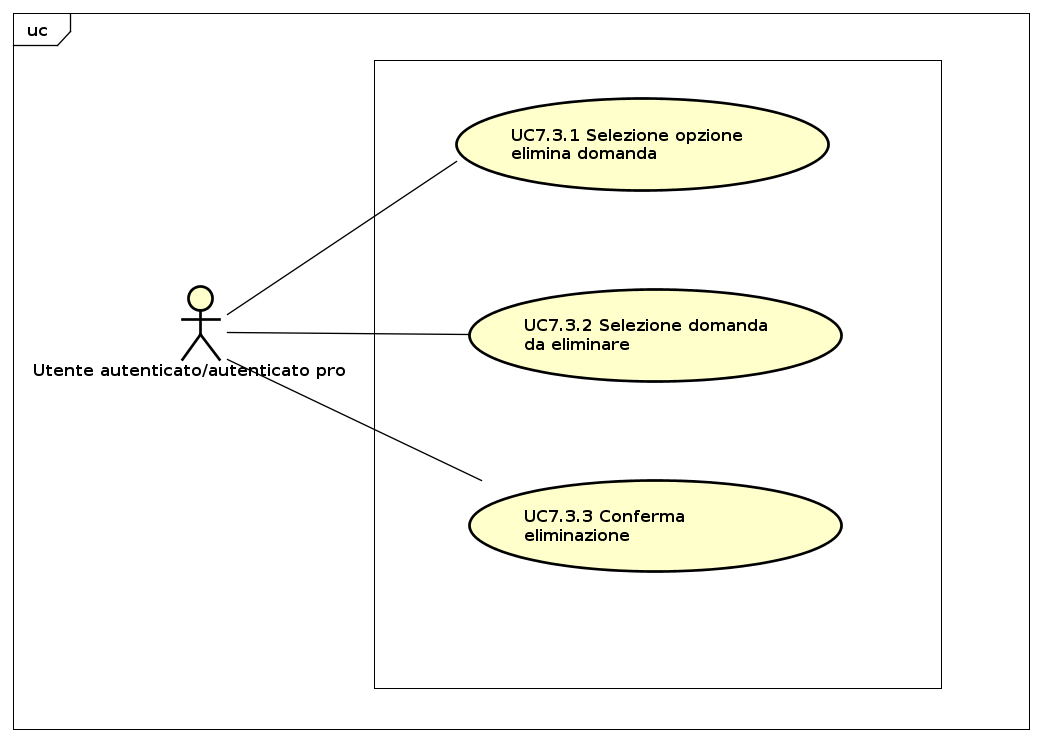
\includegraphics[scale=0.5]{UML/UC7.3.png}
	\end{center}
	\begin{itemize}
		\item
			\textbf{Attori}: utente autenticato, utente autenticato pro;
		\item		
			\textbf{Scopo e descrizione}: L'utente autenticato elimina una domanda, da lui in precedenza creata, per motivi validi e giustificati;
		\item
			\textbf{Pre-condizione}: L'utente è autenticato presso il sistema;
		\item
			\textbf{Flusso principale degli eventi}:
	       		\begin{enumerate}
					\item 	
					L'utente seleziona l'opzione per l'eliminazione di una domanda [UC7.3.1];
					\item
					L'utente seleziona la domanda da eliminare tramite uno strumento di selezione presentato dal sistema [UC7.3.2];
					\item
					L'utente conferma l'eliminazione della domanda [UC7.3.3];
	 			\end{enumerate}
		\item
			\textbf{	Post-condizione}: L'utente riceve conferma dell'avvenuta eliminazione.
	\end{itemize}
	\subsubsection{UC7.3.1 - Selezione opzione eliminazione domanda}
	\begin{itemize}
		\item
			\textbf{Attori}: utente autenticato, utente autenticato pro;
		\item
			\textbf{Scopo e descrizione}: l'utente autenticato seleziona l'opzione per compiere l' eliminazione di una domanda;
		\item		
			\texbf{Pre-condizione}: il sistema presenta all'utente autenticato l'opzione per compiere questa operazione;
		\item
			\texbf{Post-condizione}: il sistema presenta all'utente autenticato lo strumento di selezione della domanda da eliminare.
	\end{itemize}
	\subsubsection{UC7.3.2 - Selezione domanda da eliminare}
	\begin{itemize}
		\item
			\textbf{Attori}: utente autenticato, utente autenticato pro;
		\item
			\textbf{Scopo e descrizione}: l'utente autenticato seleziona, tramite uno specifico strumento presentato dal sistema, una domanda da eliminare;
		\item		
			\texbf{Pre-condizione}: il sistema presenta all'utente autenticato il modulo per modificare la domanda selezionata;
		\item
			\texbf{Post-condizione}: i campi dati del modulo di modifica, già precompilati con i dati della domanda selezionata, sono modificati.
	\end{itemize}		
	\subsubsection{UC7.3.3 - Conferma eliminazione}
	\begin{itemize}
		\item
			\textbf{Attori}: utente autenticato, utente autenticato pro;
		\item
			\textbf{Scopo e descrizione}: l'utente autenticato conferma l'eliminazione della domanda dal sistema;
		\item		
			\texbf{Pre-condizione}: il sistema presenta all'utente autenticato l'opzione per compiere questa operazione;
		\item
			\texbf{Post-condizione}: il sistema ha eliminato la domanda dal sistema.
	\end{itemize}	